\documentclass[conference]{IEEEtran}
\IEEEoverridecommandlockouts
\usepackage{cite}
\usepackage{amsmath,amssymb,amsfonts}
\usepackage{graphicx}
\usepackage{textcomp}
\usepackage{xcolor}
\usepackage{url}
\usepackage{tikz}
\usetikzlibrary{arrows.meta,positioning}
\def\BibTeX{{\rm B\kern-.05em{\sc i\kern-.025em b}\kern-.08em
    T\kern-.1667em\lower.7ex\hbox{E}\kern-.125emX}}
\begin{document}

\title{VR Climate Simulator: A Virtual Reality Testbed for\\
Studying Everyday Pro-Environmental Choices}
\author{\IEEEauthorblockN{Alessandro Tomaiuolo}
\IEEEauthorblockA{
alessandro.tomaiuol2@studio.unibo.it \\
}
\and
\IEEEauthorblockN{Gianluca Di Giacomo}
\IEEEauthorblockA{
gianluca.digiacomo@studio.unibo.it \\
}
}

\maketitle


\section{Introduction}
Individual daily routines contribute substantially to household energy use and
waste, but their effect is invisible at the moment the choice is made.
Information campaigns alone often fail to change behaviour, a phenomenon known
as the intention--behaviour gap. Immersive virtual
environments are a promising medium to close this gap, because they let people
act in a believable setting and observe the consequences of their actions in a
compressed time frame.

VR Climate Simulator is a prototype built around this idea. The user wears a
head-mounted display, watches a short introductory video,
enters a user name  and then goes through a fixed
sequence of six tasks inside an apartment. Five of the tasks are scored; the
sixth is a transition between morning and evening. The sum of the points
determines the state of the outside world, from sunny to stormy, and a
radio in the apartment comments on the situation. The world has three states,
but with the default settings only three of them can be reached (see
Section~\ref{sec:impl}).

The project has two goals. The first is experiential: to make the link
between small choices and the state of the world tangible. The second is
methodological: the application is designed as a \emph{testbed}. Choices,
timing and fine-grained actions (for example, every single piece of waste
thrown in a bin) are written to a log, and the main parameters of the
experience can be changed with little or no code. This makes it possible to
compare conditions, such as with or without the introductory video, or with
or without explicit score feedback, as discussed in
Section~\ref{sec:studies}.

The contributions of this work are: (i) a modular, data-driven architecture for
sequences of binary eco-choices with world feedback; (ii) a working VR
implementation with six tasks and three interaction techniques; (iii) a
logging pipeline suitable for between- and within-subject experiments; and
(iv) a catalogue of studies that the prototype can support.


\section{System Architecture}\label{sec:arch}

\subsection{Overview}
The application is a Unity project targeting OpenXR-compatible PC headsets.
It is organised in four cooperating layers, shown in Fig.~\ref{fig:arch}:
the \emph{player rig} (input and interaction), the \emph{task scripts}, a
central \emph{TaskManager}, and two consumers of the TaskManager, namely the
\emph{world feedback} and the \emph{session and data} layer.

\begin{figure}[htbp]
\centering
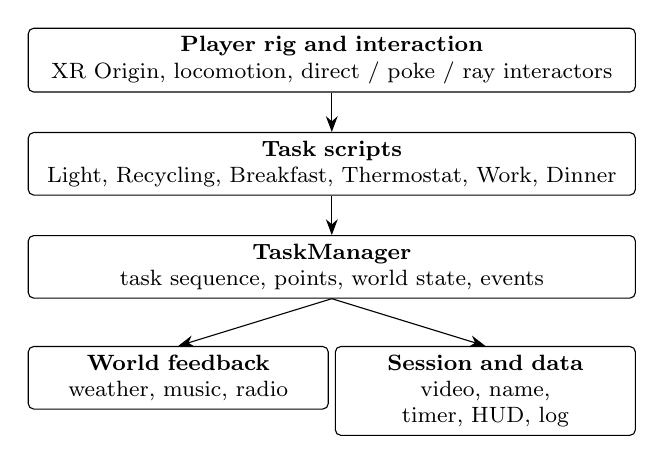
\begin{tikzpicture}[
  box/.style={draw, rounded corners=2pt, align=center, font=\footnotesize,
              text width=7.5cm, inner sep=3pt},
  half/.style={draw, rounded corners=2pt, align=center, font=\footnotesize,
              text width=3.6cm, inner sep=3pt},
  arr/.style={-{Stealth[length=2mm]}}]
\node[box] (rig) {\textbf{Player rig and interaction}\\
XR Origin, locomotion, direct / poke / ray interactors};
\node[box, below=0.5cm of rig] (tasks) {\textbf{Task scripts}\\
Light, Recycling, Breakfast, Thermostat, Work, Dinner};
\node[box, below=0.5cm of tasks] (tm) {\textbf{TaskManager}\\
task sequence, points, world state, events};
\node[half, anchor=north] (fb) at ([xshift=-1.95cm,yshift=-0.6cm]tm.south)
{\textbf{World feedback}\\ weather, music, radio};
\node[half, anchor=north] (sd) at ([xshift=1.95cm,yshift=-0.6cm]tm.south)
{\textbf{Session and data}\\ video, name, timer, HUD, log};
\draw[arr] (rig) -- (tasks);
\draw[arr] (tasks) -- (tm);
\draw[arr] (tm.south) -- (fb.north);
\draw[arr] (tm.south) -- (sd.north);
\end{tikzpicture}
\caption{High-level architecture of the application.}
\label{fig:arch}
\end{figure}

\subsection{Data-driven task sequence}
Each task of the day is described by a \texttt{TaskData} asset
(name, description and completion flag). The \texttt{TaskManager} holds the
\emph{ordered list} of these assets and exposes the current task. A task
script only does three things: it waits until its task is the current one,
it detects the user's choice, and it reports the result to the manager
(adding or removing points and marking the task as completed). Because the
order is a plain list, tasks can be reordered, removed or counterbalanced
without code changes.

\subsection{Scoring and world state}
Points are stored in the \texttt{TaskManager} and mapped to a five-level world
state by two thresholds, a good and a bad one; the two intermediate states
start at half of each threshold (Table~\ref{tab:state}). The mapping is evaluated
every time the score changes; a state change fires an event that the feedback
components listen to. All task choices change the score by the same amount
(10 points), so the weight of a single decision is a single parameter.

\begin{table}[htbp]
\caption{World state as a function of the score $p$ (default thresholds $\pm10$)}
\label{tab:state}
\begin{center}
\small
\begin{tabular}{|l|l|}
\hline
\textbf{State} & \textbf{Condition} \\
\hline
Good & $p \ge 10$ \\
Neutral\_Good & $5 \le p < 10$ \\
Neutral & $-5 < p < 5$ \\
Neutral\_Bad & $-10 < p \le -5$ \\
Bad & $p \le -10$ \\
\hline
\end{tabular}
\end{center}
\end{table}

\subsection{World feedback}
Three independent components react to the state: a weather manager (rain,
fog, skybox and exterior props), a background music manager (one track for
good, neutral and bad conditions, which is attenuated while the radio speaks)
and a radio that plays one of five spoken bulletins, one per state. The radio
is triggered at task boundaries and plays only when the state has actually
changed since the last bulletin, so that the user does not hear the same
message repeatedly.

\subsection{Session and data layer}
A session starts with an introductory video, followed by user name entry.
Only after the name is confirmed does the session timer start and the logger
begin to write. A head-up display (HUD) attached to the camera shows the
score, the elapsed time, the current task with its description and a reminder
of the two controller buttons. At the end of the last task a summary panel
lists the time spent on each task and the total time.

\section{Implementation}\label{sec:impl}

\subsection{Technology}
The prototype is implemented in Unity 6 (6000.3) with the Universal Render
Pipeline, the Input System, TextMeshPro, the XR Interaction Toolkit
(version 3.4) and OpenXR. It targets OpenXR-compatible PC headsets and is
built as a Windows 64-bit standalone player. The code
base is organised as small, single-purpose C\# components, with
scene-specific wiring done through Unity events.

\subsection{Player rig and interaction}
The rig is a standard XR Origin. Movement uses continuous thumbstick
locomotion with snap turning. Interaction relies on three techniques:
\emph{direct} interactors on the hands, where the grip is the select action
(grab objects, press switches, turn knobs) and the trigger the activate
action (squeeze a sauce bottle, squeeze an orange); \emph{poke} interactors,
used to touch the buttons of the in-world panels; and \emph{ray} interactors,
used only for the virtual keyboard of the name prompt and disabled afterwards.
User interface events are routed to the poke and ray interactors by the
XR UI input module.

\subsection{Session flow}
\paragraph{Introductory video} A 106-second video is rendered on a screen in
front of the camera while the rest of the world is hidden and other audio
sources are muted. 
\paragraph{Name entry} Since a generic OpenXR runtime offers no system
keyboard, the prompt builds a world-space panel with an on-screen QWERTY
keyboard (Fig.~\ref{fig:name}), operated by pointing with the ray and pressing
the trigger.

\begin{figure}[htbp]
\centering
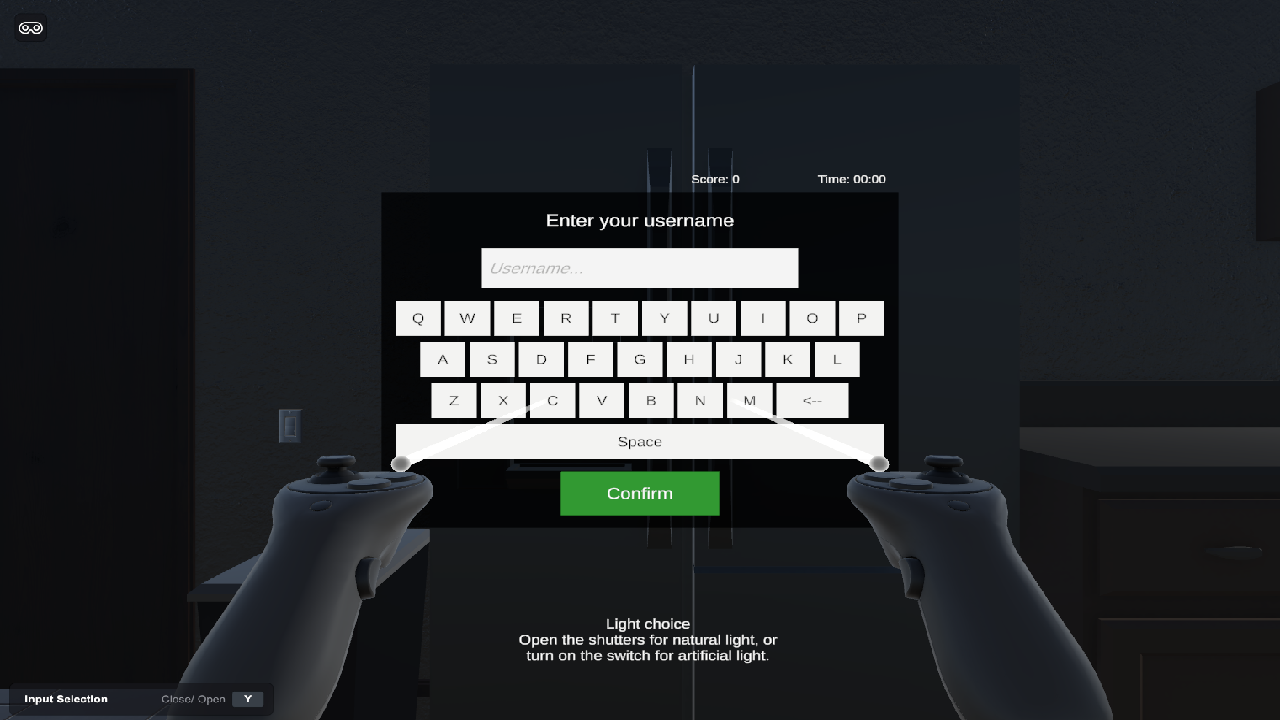
\includegraphics[width=\columnwidth]{figures/02_username_prompt.png}
\caption{User name prompt with the virtual keyboard (Unity Editor with the XR
Device Simulator).}
\label{fig:name}
\end{figure}

\subsection{The six tasks}
Table~\ref{tab:tasks} summarises the tasks, in the order in which they are
presented, and their scoring. Interactions are physical: the user reaches for
objects instead of choosing from a menu, except for the explicit decision
points, which are in-world panels (Fig.~\ref{fig:breakfast} and
Fig.~\ref{fig:thermo}).

\begin{table}[htbp]
\caption{Tasks, options and score (points)}
\label{tab:tasks}
\begin{center}
\footnotesize
\begin{tabular}{|p{1.3cm}|p{4.3cm}|p{1.8cm}|}
\hline
\textbf{Task} & \textbf{Options} & \textbf{Points} \\
\hline
Light choice & Open both window shutters (natural light) \emph{or} turn on the
switch (artificial light) & $+10$ / $-10$ \\
\hline
Recycling & Sort 15 pieces of waste into glass, paper, plastic or general
waste bins & $+10$ if sorting score $\ge 0$, else $-10$ \\
\hline
Breakfast & Make a breakfast (orange juice and jam toast) \emph{or} eat a
snack (at least 5 items), then touch the bell & $+10$ / $-10$ \\
\hline
Thermostat & Turn the thermostat off \emph{or} leave it on & $+10$ / $-10$ \\
\hline
Dinner & Order a pizza and soda \emph{or} cook a burger following a recipe &
$+10$ / $+10$ \\
\hline
\end{tabular}
\end{center}
\end{table}

\paragraph{Light choice} Both window shutters must be fully opened to confirm
the natural option; pressing the lamp switch confirms the artificial one. The
first decision locks the other controls.

\paragraph{Recycling} The waste items are instantiated at dedicated spawn
points. Each item carries a material type (plastic, paper or glass). A correct
bin accepts the item and adds one point to an internal sorting score; the
general waste bin accepts anything but always subtracts one point; a wrong
differentiated bin rejects the item and pushes it back. The task ends when all
items have been disposed of. Note that metal cans are classified as plastic in
the current data, because the game has no metal bin.

\paragraph{Breakfast} The user chooses between a healthy path and a snack
(Fig.~\ref{fig:breakfast}). Food and drinks are eaten by bringing them to the
face, where a small trigger volume attached to the camera removes the object.
The task ends when the required items are consumed and the bell is touched
with a hand.

\begin{figure}[htbp]
\centering
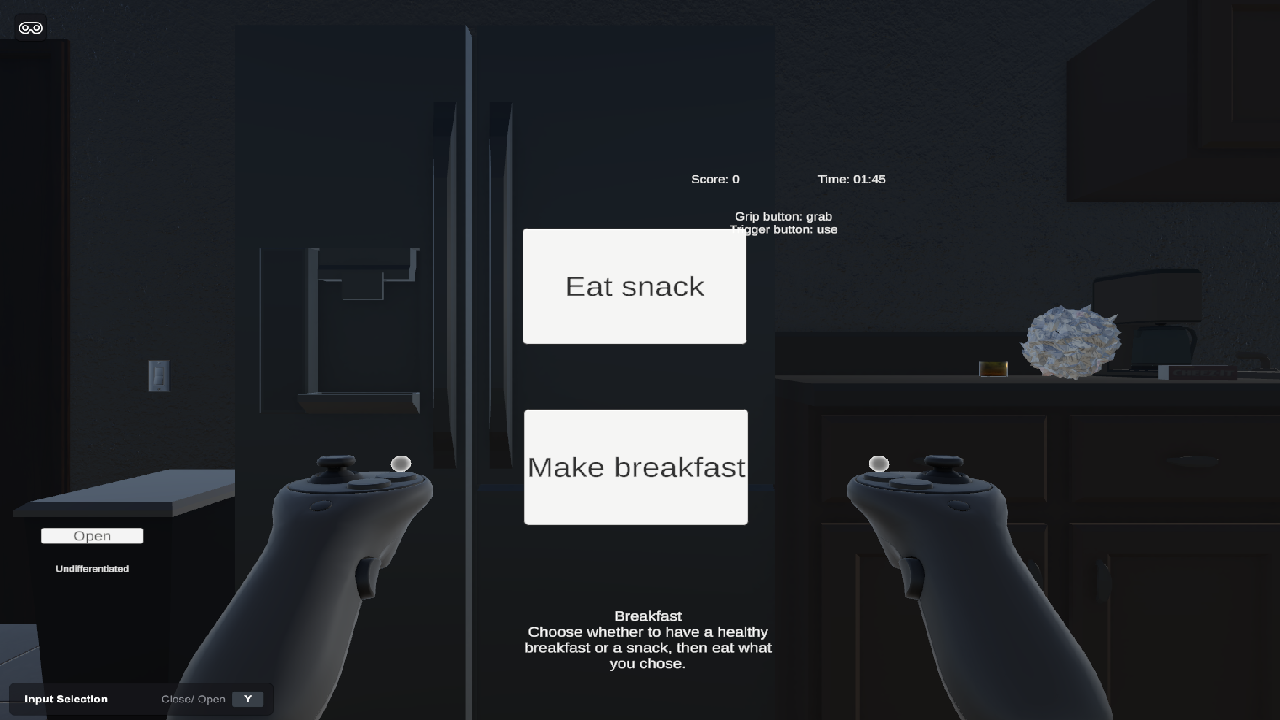
\includegraphics[width=\columnwidth]{figures/06_breakfast_choice.png}
\caption{Decision panel of the breakfast task together with the HUD.}
\label{fig:breakfast}
\end{figure}

\paragraph{Thermostat} A wall thermostat shows the temperature, can be
adjusted with two buttons and emits a continuous idle sound. Choosing to turn it off
hides the display, fades out the sound and disables the buttons
(Fig.~\ref{fig:thermo}); both choice buttons disappear after any decision.

\begin{figure}[htbp]
\centering
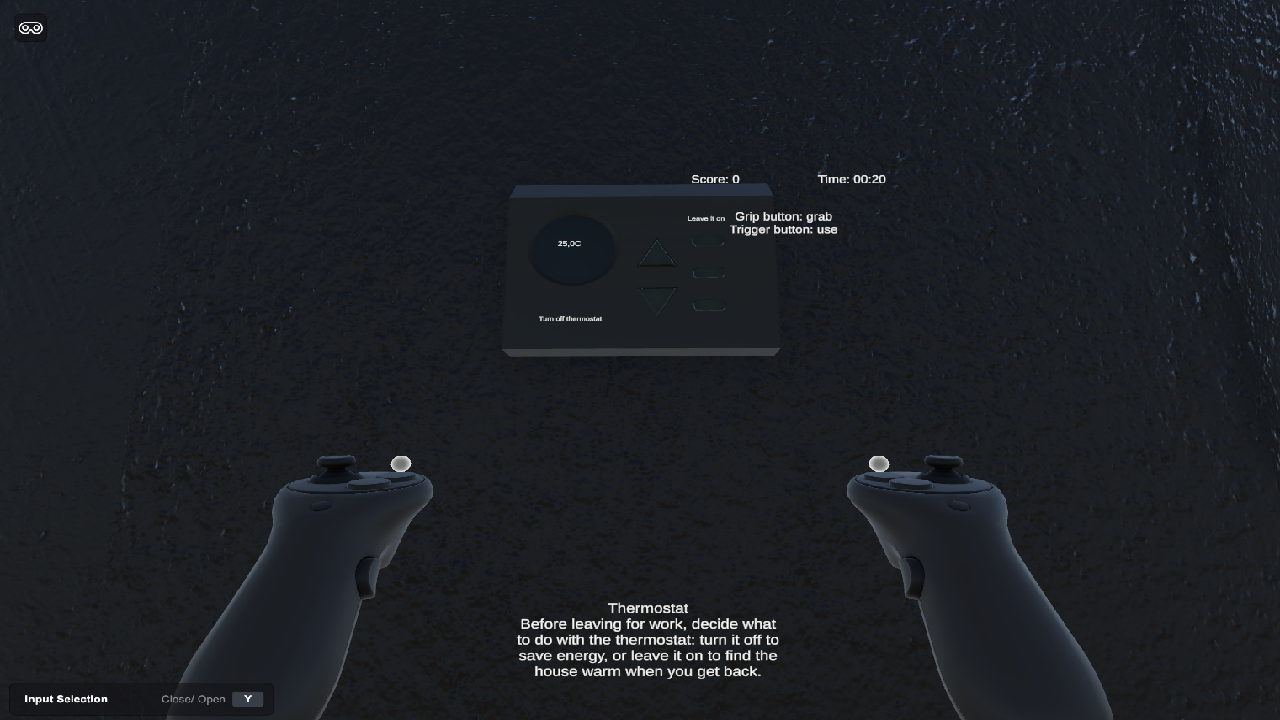
\includegraphics[width=\columnwidth]{figures/07_thermostat_choice.png}
\caption{Thermostat panel with the two choice buttons.}
\label{fig:thermo}
\end{figure}

\paragraph{Go to work and Dinner} The work task is not scored and separates
morning and evening. The dinner offers an immediate option (order) and a
procedural one (cook a burger by adding ingredients in the right order, guided
by a recipe on the wall). In the current configuration both options score
positively, so this task does not discriminate between users.

\subsection{Feedback and HUD}
The weather, music and radio components described in the previous section are
implemented as separate scripts connected to the manager's events. The HUD is
rendered on top of the scene with an always-visible text material
(Fig.~\ref{fig:hud}). The two reminder lines are task-independent: ``Grip
button: grab'' and ``Trigger button: use''.

\begin{figure}[htbp]
\centering
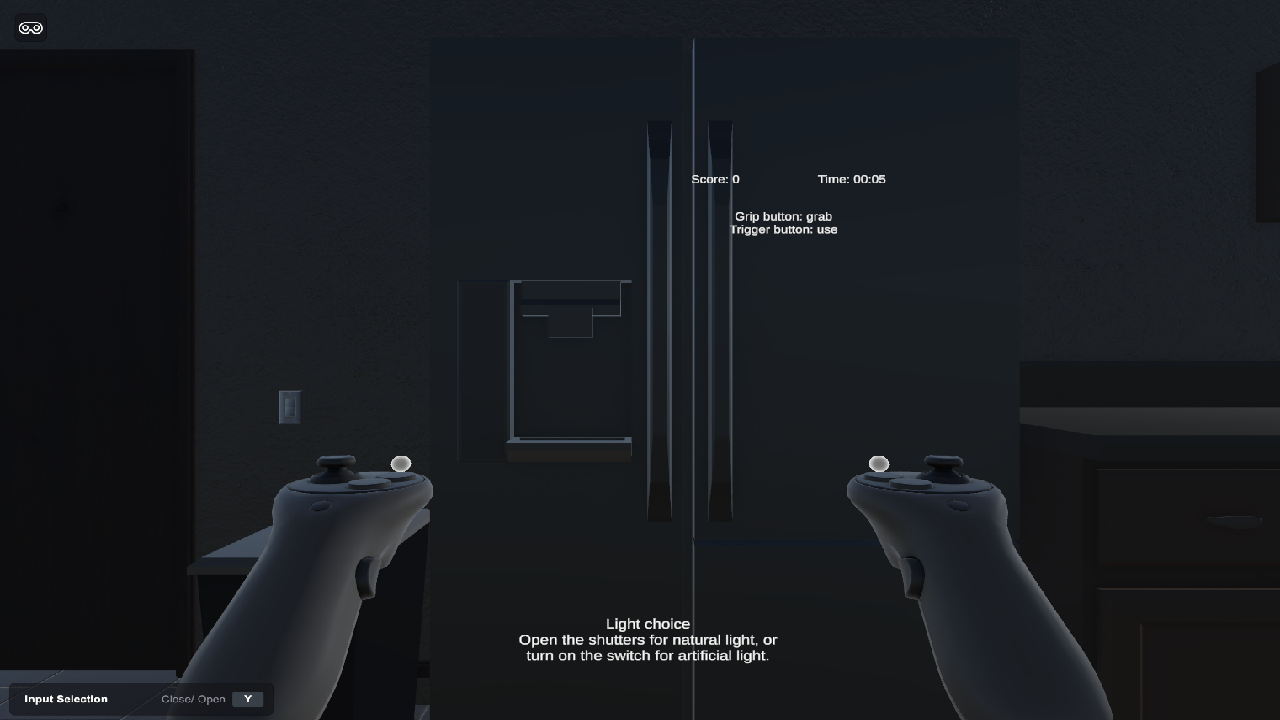
\includegraphics[width=\columnwidth]{figures/04_hud_light_task.png}
\caption{HUD with score, timer, controller hints and current task.}
\label{fig:hud}
\end{figure}

\subsection{Audio assets}
All audio content was produced with generative tools. The background music
tracks were generated with MusicFX\footnote{\url{https://musicfx.net/}}
from text prompts, one for each world condition (good, neutral and bad); the
prompts are listed in Table~\ref{tab:prompts}. The scripts of the five radio
bulletins, one per world state, were written with Gemini, and the spoken
tracks were synthesised from those scripts with ElevenLabs. \footnote{\url{https://elevenlabs.io/}}

\begin{table}[htbp]
\caption{Prompts used to generate the background music with MusicFX}
\label{tab:prompts}
\begin{center}
\footnotesize
\begin{tabular}{|l|p{5.3cm}|}
\hline
\textbf{Track} & \textbf{Prompt} \\
\hline
Good & Instrumental background music for a VR game about a healthy, thriving planet. Classical orchestration, gentle violins, soft string ensemble, and delicate piano. Featuring ambient nature sounds with clearly audible birds singing (birdsong). Peaceful, pure, serene, and calming mood. Slow tempo, bright and airy atmosphere. Seamlessly loopable, non-distracting video game soundtrack.
\\
\hline
Neutral & Instrumental background music for a VR game about nature and sustainability. Ambient lo-fi, soft acoustic guitar, gentle warm synth pads, organic textures. Chill, calm, relaxing, peaceful mood. Slow tempo, minimal percussion. Seamlessly loopable, non-distracting video game soundtrack.
\\
\hline
Bad & Instrumental cinematic background track for a VR game depicting environmental crisis. Dark ambient, industrial electronic, distorted heavy synths, deep sub-bass drones. Anxious, tense, unsettling, urgent mood. Fast tempo, driving aggressive rhythm, harsh textures, metallic clock-ticking sound effect. Seamlessly loopable, creates dread and pressure.
\\
\hline
\end{tabular}
\end{center}
\end{table}
% TODO: if useful, add the Gemini prompts and the radio scripts (e.g. in an appendix).

\subsection{Data logging}
The logger writes one row per event to a semicolon-separated CSV file stored
in a \texttt{Logs} folder next to the executable (or to the project root in the
Editor); a single file accumulates all sessions. Logged events
include task start and completion, every choice (breakfast path, thermostat
decision, light, transport, dinner), every temperature adjustment, and for
the recycling task every throw with the object, its real material, the chosen
bin and whether it was correct, including rejected attempts. Logging starts
only after the user name has been confirmed. At the end of the session the
per-task durations are shown in the summary panel (Fig.~\ref{fig:summary}).

\begin{table}[htbp]
\caption{Columns of the session log}
\label{tab:log}
\begin{center}
\footnotesize
\begin{tabular}{|l|p{5.3cm}|}
\hline
\textbf{Column} & \textbf{Content} \\
\hline
User & Name entered by the participant \\
Timestamp & Date and time with millisecond resolution \\
Task & Name of the current task \\
Action & Type of event (e.g. task started, choice, item thrown) \\
Details & Event-specific information (choice, object, bin, delta) \\
Task time (s) & Seconds since the task started \\
Score & Global score at the time of the event \\
\hline
\end{tabular}
\end{center}
\end{table}

\begin{figure}[htbp]
\centering
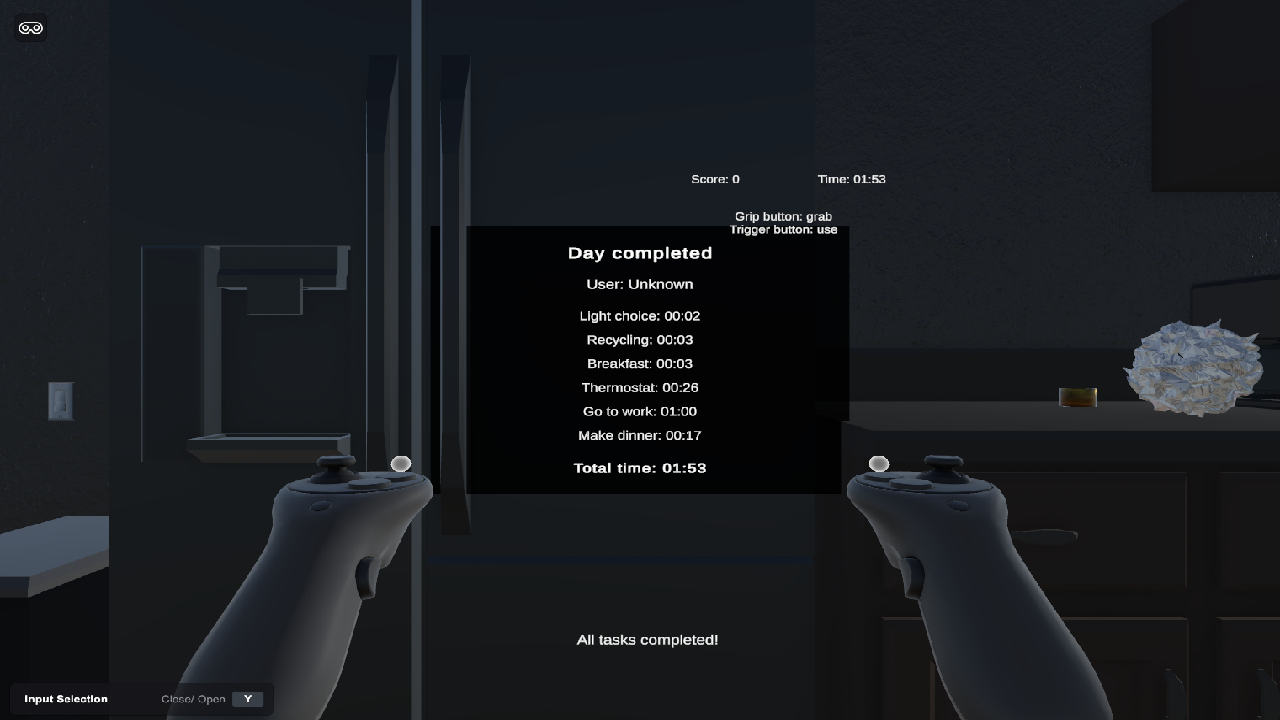
\includegraphics[width=\columnwidth]{figures/10_session_summary.png}
\caption{End-of-session summary with the time spent on each task.}
\label{fig:summary}
\end{figure}

\section{Possible Studies}\label{sec:studies}
Thanks to the data-driven design and the detailed log, the same application
supports several experiments with little or no code. Table~\ref{tab:vars}
lists the manipulable variables and where they are set.

\begin{table}[htbp]
\caption{Variables that can be manipulated with little or no code}
\label{tab:vars}
\begin{center}
\footnotesize
\begin{tabular}{|p{2.5cm}|p{5.3cm}|}
\hline
\textbf{Variable} & \textbf{How it is set} \\
\hline
Introductory video & Assign or remove the clip \\
Explicit score & Show or hide the score in the HUD \\
Feedback channels & Wire or unwire weather, music and radio in the manager's
events \\
Decision weight & Points per choice and the two state thresholds \\
Task order & Order of the task list \\
Effort cost & Items to eat at breakfast; commute duration (one constant in
the code) \\
Recycling difficulty & Number and type of items, and the available bins \\
\hline
\end{tabular}
\end{center}
\end{table}

\subsection{Measures}
The log provides, for each participant: the choice made in every task
(binary eco-choice), the time spent on each task and in total, the number of
temperature adjustments, and for recycling the full sequence of throws, from
which accuracy, error types and learning across items can be computed. The
application does not collect questionnaires; these can be administered before
and after the session and joined to the log through the user name.

\section{Conclusions}\label{sec:concl}
We presented VR Climate Simulator, a VR prototype in which small everyday
choices drive the state of a virtual world and are recorded in a detailed
log. The data-driven task sequence, the event-based feedback channels and the
logging pipeline make it a testbed for studies with little or no code..

\end{document}
